\documentclass[orivec]{llncs}
\usepackage{graphicx}
\usepackage{amsmath}			% for "cases"
\usepackage{amsfonts}		% for frakur fonts
\usepackage{mathrsfs}		% for curly "E" error symbol
\usepackage{float}
\usepackage[most]{tcolorbox}	% for wrapping example in color box
% \usepackage{wrapfig}			% wrap figure beside text, used in example
\usepackage{tikz-cd}			% commutative diagrams
\usepackage{tikz}
\usepackage{amssymb}			% for \multimap \updownarrow \bigstar \varnothing
\usepackage{sectsty}			% change section color
% \usepackage{turnstile}		% longer turnstiles
\usepackage{wasysym}			% smileys
\usepackage[normalem]{ulem}	% underline with line breaks: /uline
\usepackage{hyperref}		% refs, links become clickable
\usepackage[]{algorithm2e}	% algorithms

\usepackage{geometry}		% change paper size
\geometry{
  a4paper,         % or letterpaper
  textwidth=18cm,  % llncs has 12.2cm
  textheight=27cm, % llncs has 19.3cm
  heightrounded,   % integer number of lines
  hratio=1:1,      % horizontally centered
  vratio=2:3,      % not vertically centered
}
\usepackage[fontsize=13pt]{scrextend}

% *************** Delete when not using Chinese or colors **********************
\usepackage{xeCJK}
\setCJKmainfont[BoldFont=SimHei,ItalicFont=KaiTi]{SimSun}
\usepackage{color}
\definecolor{cerulean}{RGB}{100,100,200}
%\newcommand{\emp}[1]{\textbf{\textcolor{Cerulean}{#1}}}
\newcommand{\emp}[1]{\textbf{#1}}
\definecolor{grey}{rgb}{0.9,0.9,0.9}  % grey

% \chapterfont{\color{blue}}  % sets colour of chapters
\sectionfont{\color{blue}} 
\subsectionfont{\color{blue}} 
\subsubsectionfont{\color{blue}} 
\setcounter{secnumdepth}{3}		% use numbers in subsubsections

\let\emptyset\varnothing			% more beautiful empty set symbol
\newcommand{\vect}[1]{\boldsymbol{#1}}
\newcommand*\sigmoid{\vcenter{\hbox{
\includegraphics{sigmoid.png}}}}
\newcommand*\KB{\vcenter{\hbox{
\includegraphics{KB-symbol.png}}}}
\newcommand*\NN{\vcenter{\hbox{\includegraphics{NN-symbol.png}}}}
\newcommand*\invsigmoid{\vcenter{\hbox{\includegraphics{inverse-sigmoid.png}}}}
\newcommand{\invW}{\, \rotatebox[origin=c]{90}{W}}
\newcommand{\invw}{\, \rotatebox[origin=c]{90}{w}}
\newcommand*\rectifier{\vcenter{\hbox{\includegraphics{rectifier.png}}}}
\newcommand{\dashh}{\textemdash~}

\newcommand{\tikzmark}[1]{\tikz[overlay,remember picture] \node (#1) {};}

\renewcommand{\thefootnote}{\fnsymbol{footnote}}
\interfootnotelinepenalty=10000

% ***** Boxed variables inside math equations
% \newcommand*{\boxedcolor}{black}
\makeatletter
% \renewcommand{\boxed}[1]{\textcolor{\boxedcolor}{%
% \fbox{\normalcolor\m@th$\displaystyle#1$}}}
% \setlength{\fboxsep}{1pt}
\renewcommand{\boxed}[1]{\fbox{\m@th$\displaystyle\scalebox{0.9}{#1}$} \,}
\makeatother

\overfullrule=0mm

\newsavebox{\MyName}
\savebox{\MyName}{
\includegraphics[scale=0.6]{YKY.png}}

\title{什么是遗传/进化算法? (What are evolutionary algorithms?)}
\titlerunning{什么是遗传/进化算法?}
\author{\usebox{\MyName} (King-Yin Yan)
% \\ \footnotesize{General.Intelligence@Gmail.com}
}
\institute{General.Intelligence@Gmail.com}

\begin{document}

\maketitle
\setlength{\parindent}{0em}
% \setlength{\parskip}{2.8ex plus0.8ex minus0.8ex}
\setlength{\parskip}{2.8ex}

%\begin{abstract}
%\end{abstract}

这是基於 \textbf{进化论} 而启发出来的一种很特别的 \textbf{机器学习} 技巧。  在人工智能中有三大重要技巧: 逻辑、神经网络、和进化算法。   原来 Alan Turing 很早就看到 进化 和 machine learning 之间有明显关系,而现时机器学习的一个很有名的研究者 Leslie Valiant 也在 \href{http://book.douban.com/subject/20016696/}{新书} \href{http://www.amazon.com/Probably-Approximately-Correct-Algorithms-Prospering/dp/0465060722/ref=sr_1_1?ie=UTF8&qid=1426558262&sr=8-1&keywords=probably+approximately}{(English version)} 中谈论这课题。

\section{进化论}


首先,要理解什么是进化论。  举例来说,假设某只动物的基因变异 令牠比同伴有更锋利的爪和牙齿,那么那牠就能吃到同伴吃不到的食物,也能抢到更多异性去交配。  久之,牠的同伴会较少后裔、甚至绝种,而牠的后裔则会越来越强盛。  这就是「物竞天择 适者生存」。

人类的情况有些不同,因为人类有 \textbf{文化} (意即靠语言传授下来的那些知识),所以有些优点不是纯粹由基因可以看出来。  说到这个问题很具争议性,因为涉及优生学等道德议题。  人们喜欢举反例,例如说『这个男生长得不好看 却有很多女朋友』等等,我不想扯得太远。  想想看,人类最强烈的感情,莫过於找不到伴侣传宗接代,而我们得不到异性的青睐 就会很痛苦,或者看到别人有更多「资源 resource」会妒忌,这些都是进化很有力的证据。 人类的感情通常可以用进化解释,这科目叫 evolutionary psychology (进化心理学)。

我个人认为,竞争是生物界以至人类社会的基本状况,我们必须接受并习惯它。  人类在商业、战争、体育、文艺、甚至下棋也是在竞争。   \textit{天行健 ~ 君子以自强不息},那是很好的勉励。

\section{进化学习}

以前说过,机器学习的目的就是要在浩瀚的 \textbf{假设空间} (hypothesis space) 中寻找那些能正确地解释现实的语句。  例如婴孩可能用「有胡子就是爸爸」 来解释身边出现的人。

问题是假设空间太大,我们如同「在禾秆推里找一只针」,单靠 brute force 不是办法。

进化算法就是在很大的空间里 寻找某个 \textbf{最佳答案} (optimal solution) 的一个很强的技巧。 它把需要寻找的 candidates 模拟成一个「人口」population,任由这些 candidates 在某个人工的环境下竞争, 然后,每次选取得分最高的一小撮样本,让它们「交配」,即 \textbf{基因重组} (genetic recombination),那样产生新一批的  candidates, 如此逐步推向越来越优秀的 solutions。

举个例子,研究者用进化算法进化出一些电子电路,例如用於音响的滤波器 (filter) ,其 performance 甚至比人手设计的还要优越。  而且,那电路很不规则而且难理解,人们不知道它是如何运作的,有些部分甚至有多馀的元件存在。  那是因为进化的过程中,有时一些表面上没用的「器官」在组合之后或许变有用,所以进化的结果也常保留很多「废物 junk」。

我曾经想用这方法去写 logic-based AI 的学习功能(我们要进化的 candidates 就是那些 \textbf{逻辑句子} logic formulas)。

\section{Algorithm}

\subsection{具体的算法怎样?}

\let\labelitemi\labelitemii
\begin{itemize}
\item 初始时,预备一个 population,可以是随机产生的。
\item 对每个 candidate 进行 \textbf{估值} (evaluation),即是让这个 candidate 在人工的世界里生存。  例如我们测试它在所需的功能的表现如何。  那计分的方法叫 \textbf{objective function} 「目的函数」。
\item 选取表现最好的 N 个 candidates,进行 \textbf{变种} (mutation) 或 \textbf{重组} (recombination)。  变种是作用在单个 candidate 上的,重组则需要一对 candidates。  那就涉及到我们怎样将设计空间的元素表示为「基因」,於是有所谓 \textbf{表述} (representation) 的问题。  这编码是要由研究者设计的。
\item 在评分的时候,可以容许那些 candidates 在环境中互相 \textbf{合作} 亦同时竞争,那叫 cooperative evolution。   我觉得 logic-based AI 有需要用这方法,因为在知识库中的每个知识片段,是要和其他知识互相作用,那逻辑系统才能推导出有意思的结果。  
\end{itemize}

\href{http://www.cleveralgorithms.com/}{这本书(作者的网站免费提供在线阅读)} 深入浅出地介绍了几个「nature-inspired」算法:
\begin{equation}
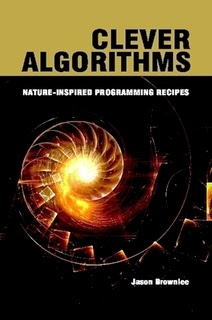
\includegraphics[scale=0.75]{clever-algorithms-cover.jpg}
\end{equation}

例如这个 \href{http://www.cleveralgorithms.com/nature-inspired/evolution/genetic_algorithm.html}{基因算法 的程式},用 Ruby 写成,只需短短一页。


\section{实习}


那个例子叫 "OneMax",每个个体是一串 0 和 1 的字串,目标是全部变成 "1"。

这个例子特别简单,因为「基因」就是个体的 \textbf{显形} (phenotype),省略了 \textbf{基因表述} (gene expression) 这步骤,便於学习。

实际运行时,发生了有趣的现象。  我先试 Ruby,然后把它翻译成 Scala,但奇怪地 Scala 版本的运行没有收敛到完美的结果,而 Ruby 版本很快就达到了。

我把 Ruby 和 Scala 进化的两个 populations 用图像显示出来,每一横列是一个个体。  第一片段是 Ruby「正常」的进化(到结尾时已经进化出第一个完美的纯 "1" 个体):

\begin{equation}

\includegraphics[scale=0.5]{video-thumbnail.png}
\end{equation}

第二个是我写的 Scala 「不正常」进化:
\begin{equation}

\includegraphics[scale=0.5]{video-thumbnail.png}
\end{equation}

可见在病态版本,那些孩子逐渐变成一模一样,而且每个也有同样的缺陷(因而显示成垂直线) 。

为什么呢?  Debug 了整整两天,才发现一个把 0 写作 1 的错误,令到那个 point mutation 的函数形同虚设,亦即是说 病态版本 根本缺乏 point mutations。

那是一个非常有启发性的 bug,使我学到了,单是 sexual reproduction 还不能做到高效率的进化,原来个体的 point mutations 也有关键的重要性,而我一直误以为 \textbf{有性生殖} 是产生 \textbf{多样性} (diversity) 的唯一途径。  我依稀记得文献里曾提及这点,但不记得了。  有趣吗?  {\Large \smiley}

\quad \quad \quad --- 完 ---

\bibliographystyle{plain} % or number or aaai ...
\bibliography{AGI-book}

\end{document}
